% This is a sample LaTeX input file.  (Version of 12 August 2004.)
%
% A '%' character causes TeX to ignore all remaining text on the line,
% and is used for comments like this one.

\documentclass{article}      % Specifies the document class

                             % The preamble begins here.
\title{SKBD: Segment Knotting Boundary Detection For Room Layout Detection}
\author{Barna Mikler, Botond Geonczeol, Dominik Li, \\ Matyas David, Balint Boros}
\date{September 25, 2024}

\newcommand{\ip}[2]{(#1, #2)}
                             % Defines \ip{arg1}{arg2} to mean
                             % (arg1, arg2).


\usepackage[backend=biber, style=numeric]{biblatex} % For references
\addbibresource{references.bib}
\usepackage{hyperref}
\usepackage{graphicx}                               % For including images
\usepackage{subcaption}                             % For subfigures
\usepackage{algorithm}
\usepackage{algpseudocode}
% Set the page and margin size
\usepackage[letterpaper,top=2cm,bottom=2cm,left=3cm,right=3cm,marginparwidth=1.75cm]{geometry}
\begin{document}             % End of preamble and beginning of text.

\maketitle                   % Produces the title.

Image-based room layout reconstruction aims to predict the spatial structure of a room from a small number of images. Most previous papers relied on heavy assumptions of the layout, i.e. the room having a cuboid shape, a single ceiling and a single floor. Our work focuses on improving the predictions for rooms that does not satisfy these restrictions. This is achieved with the help of our Segment Knotting Boundless Detection System (SKBDS). This method detects the connection of segments without heavily relying on their proximity. The experimental results demonstrate that our system vastly outperforms current state-of-art methods on datasets consisting of rooms with unusual layout, but it also performs similarly to them on regular datasets.


\section{Introduction}

\subsection{The general reconstruction of room layouts} %Problem statement
A reconstruction of a room is the process of taking in some data from an empty room and transforming it into its 2D floor plan. The floor plan contains basic information, such as the overall shape of the room as well as the location of windows and doors. The spatial dimensions can also be noted down, including the length of a wall or the height of the room. This floor plan is useful in many applications and services, such as virtual room design or simple information gathering in a faster, more convenient way. 

The efficient and precise reconstruction of a room has been attempted numerous
times. The data in most cases is comprised of one or more images taken of the room from various spots. The process of transformation is the presented problem, for which this paper attempts to provide a general solution to. The problems lie in the shape of a given room and how variable any room really is. Given that this problem is solved and the process is complete for any room, many new applications can emerge that utilize this process and make way for new services. The floor map would be more readily available with just a few images taken of the room. This would absolve the need for the task of creating these floor plans by hand, making the process more efficient as a result.

\subsection{The problem with reconstruction of non-cuboid spaces} %Motivation
For most rooms, we can differentiate between cuboid and non-cuboid shaped instances. a cuboid room is regular and rectangular, while a non-cuboid room can have irregular, curved, or non-right-angled surfaces. These differences are presented in Figure\ref{fig:bothfigures} In the realm of cuboid shaped rooms, some progress has been made with the goal of reconstructing. However, there is need for a less restrictive and overall more general process that is able to reconstruct rooms, regardless of shape. Is there maybe a more efficient and general process for reconstruction? This is the question we put the emphasis on in this paper.

\begin{figure}[htbp]
    \centering
    \begin{subfigure}[b]{0.38\textwidth}
        \centering
        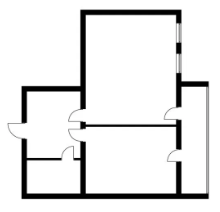
\includegraphics[width=\textwidth]{images/cuboidfloorplan.png}
        \caption{Example of cuboid rooms}
        \label{fig:cuboidroom}
    \end{subfigure}
    \hfill
    \begin{subfigure}[b]{0.38\textwidth}
        \centering
        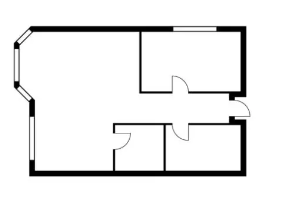
\includegraphics[width=\textwidth]{images/noncuboidfloorplan.png}
        \caption{Example of non-cuboid room (far left)}
        \label{fig:noncuboidroom}
    \end{subfigure}
    \caption{Difference in room shapes}
    \label{fig:bothfigures}
\end{figure}

This is a difficult problem for the following reasons. A room can take on different shapes, the room height can change and in some places the space can even narrow or widen. For this reason it has been proven to be a difficult challenge to efficiently map out a room's floor plan based on images. The difficulty is compounded when relying on one image to extract spatial information. Images provide limited depth perception when taken from a single viewpoint. This also makes the scaling of a processed room difficult to evaluate.

\subsection{Image descriptors}
This paper utilizes image descriptors. These are numerical representations of a feature on an image region. The region can be the whole image, when this is the case the descriptor is called a global descriptor. When an image region is a subset of the image, it is called a segment of the image. When a descriptor only retrieves information from a segment, it is called a local descriptor.

Descriptors can also be broken down into multiple types based on the feature they focus on. We mainly used the general information descriptors that describe one basic characteristics of an image. A characteristic can be for example color, shape or texture. During our solution we frequently relied on local descriptors that extract a single characteristic from a segment. These descriptors are also used to identify segments in a given image, like the SIFT \cite{lowe2004distinctive} and SURF \cite{speeduprobustfeatures}. More information about descriptors can be found in the book Introduction to MPEG 7: Multimedia Content Description Language\cite{manjunath2002mpeg7}.




\subsection{The Basis of SKBD} %Solution
There are various attempts at resolving the problem of room reconstruction. Most papers in this field are concerned with the reconstruction of cuboid shaped rooms with information given from a single image. As a consequence, these results provide a limited precision on depth and scaling. The most promising papers are given more attention in Related Work[\ref{sec:relatedwork}]

Our presented solution, named Segment Knotting Boundary Detection (abbreviated to SKBD) aims to provide a more versatile method for reconstructing a room. With this paper, the aim was to develop a processing method that can reconstruct a non-cuboid shaped room from a small number of images. The solution can also determine the depth and scale properties of a room, since multiple viewpoints are being used. It also puts more emphasis on detecting segments outlined by feature points and segments detected by local descriptors. 

\subsection{Segment connection} %Contributions
This solution differs from the currently published ones in terms of usage and in terms of the reconstructing process. A heavy focus was put on image segmentation. A segment refer to a part of the image that can be detected and separated. Detecting the connection between segments involves identifying how these segments relate to one another. This could mean determining if they belong to the same structure, if they interact in some way, or if they share common features. SKBD relies on detecting segments in the taken images and then matching them. Using this approach we relied less on the proximity of these segments which in turn resulted in identifying connections that may not be immediately obvious.

%Roadmap
This article will discuss related works [\ref{sec:relatedwork}] in this field, explains the methodology and development process of SKBD, then presents findings about the accuracy of the developed method. It will also draw a conclusion based on the results of the development and talk about potential directions for this method in the future.


\section{Related Work}
\label{sec:relatedwork}

Several papers focus on the topic of room layout estimation, with multiple
different approaches to the problem. Most existing methods tackle this problem
with strict assumptions, such as modeling the room by a parametric box (cuboid)
or assuming the room has a single-foor single-ceiling construction.

\paragraph{}

\textbf{Layout Estimation Using Geometric Hints} Room Layout Estimation Using
Geometric Hints\cite{8451365} aims to predict surface layout from a single image
by utilizing a deep network that combines textures and geometric hints. 
Ruifeng et al. \cite{8451365} have presented the use of a multi-scale 
Convolutional Neural Network (CNN) approach which incorporates a multi-channel
Fully Convolutional Network (FCN).
Their method works by assigning a surface label of the five possible surfaces to
every pixel of the input image, and then utilizing a depth- and a normalmap
generated using these labels to determine which part of the image is predicted to
belong to which surface. Under the Manhattan world assumption\cite{790349} only
these five surfaces \{Left, Front, Right, Ceiling, Ground\} can be visible in an
image at the same time. After extracting the depthmap and the normalmap with the
method described above, they used these as additional channels alongside the RGB
pixel values of the image as the input of their multi-channel FCN.

\paragraph{}

\textbf{Layout Estimation Using Undirected Graph}
Undirected graph representing strategy for general room layout estimation\cite{YAO2023103963}
paper details a process that focuses on the use of undirected graphs. It parameterizes the layout to a graph, where layout vertices are regarded as the graph's vertices. A neural network then processes this graph and gives the layout as the result. This layout consists of the detected vertices and therefore, the visible walls, the floor and ceiling are also detected. This article also builds on the Manhattan world assumption\cite{790349}, therefore the same rules apply here as well. Subsequently, both cuboid and some non-cuboid shaped rooms were succesfully processed, although only limited information was extracted.

\paragraph{}

\textbf{Learning to Reconstruct 3D Non-Cuboid Room Layout from a Single RGB Image} Learning to Reconstruct 3D Non-Cuboid Room Layout from a Single RGB Image\cite{9707088} presents a novel approach to reconstructing the 3D layout of indoor scenes, including walls, ceiling, and floor, from a single RGB image, addressing limitations of previous cuboid-based methods that lack flexibility in real-world scenarios. By framing room layout estimation as a plane detection problem, the proposed framework integrates the geometric relationships between detected 3D planes and 2D vertical lines of adjacent walls. This allows the method to discern whether walls are physically connected or disconnected in 3D space, utilizing Convolutional Neural Networks (CNNs) to detect both planes and vertical lines while estimating the 3D parameters for each plane.

\paragraph{}

\textbf{Polygon Detection for Room Layout Estimation using Heterogeneous Graphs and Wireframes}
This paper \cite{10350607} presents an advanced method for creating 2-dimensional room layouts from photos by leveraging cutting-edge neural network techniques and geometric reasoning. It introduces a Heterogeneous Graph Transformer (HGT) model that excels in detecting planes, lines, and junctions in images, representing these projections as polygons to generate accurate room layouts. By avoiding traditional constraints like cuboid room shapes, the method can handle more complex environments. Additionally, the model directly estimates room layouts without the need for post-processing heuristics, achieving superior performance in key metrics compared to state-of-the-art methods. Its ability to accurately project 3D planes into 2D, along with thorough evaluations using synthetic and real wireframe detections, makes this approach highly effective for producing detailed, accurate 2D floor maps from simple images.

\paragraph{}

\textbf{DALSM: A Direction-Aware Line Segment Matching Method}
Line segment matching is essential in tasks like 3D reconstruction, image stitching. Traditional methods rely on feature point correspondences to estimate projective transformations between images. However they often overlook important attributes like intensity and gradient, leading to inaccurate matches. Descriptor-based methods, such as Line Band Descriptor (LBD), address this by analyzing detailed image features, but their complexity can make them impractical for real-time applications and we might not have as detailed images as input.

To improve accuracy, the proposed Direction-Aware Line Segment Matching (DALSM) method incorporates direction-aware attributes, such as intersection angles and gradient directions, along with feature point correspondences. This approach enhances precision without increasing computational costs. DALSM can be useful in generating floor plans from 1-2 images, as it reliably matches line segments representing walls and floors giving more precise layout estimations.

\section{Methodology}
\label{sec:methodology}

\subsection{Previous Attempts} %Tried methods
At first, we tried to rely solely on descriptors. The first proposed method was a combination of local and global descriptors that describe various features on the images. We used the SIFT, ORB and SURF descriptors that are local descriptors. Then, using global descriptors we tried to tie the identified segments together. These alone however were not sufficient. This method was unable to capture a more significant connection between the separate images and therefore was not able to be used to reconstruct the room itself. An underlying problem of this method was that local and global descriptors capture different types of information, which are not easily associated with one another.

A different method tried was the involvement of a machine learning model with a well-trained CNN. We hoped that there were some hidden connection points that are accurately detectable using a neural network. This produced some results, however the use of this model was limited only to a set of cases. In these cases the image sets exceeded the minimal amount of images needed to map out a room with no blindspots. Most image sets consisted of images that had many repeating regions in them, which in our study is a redundant set. We aim to process and reconstruct a room with as few images as possible and minimal amount of repeating image regions.   

A purely algorithmic approach was also tried. There were some promising results using graphs and edge detection. Using this method, we detected the edges of all walls with a modified version of Harris-Corner detection. Then, the developed algorithm managed to connect all corners of a non-cuboid shaped room using graph theory. This ended up not fitting our study, since detecting only the edges of a room is not enough to fully detail it. Therefore, the full recostruction of a room was determined to be impossible using this method. This method took some inspiration from \cite{9707088}, as this paper also used a similar method to determine edges of a room.


\subsection{Detection of distinct segments} %Segment detection
For segment detection, we revisited local descriptors. Using these descriptors we were able to detect spots in the image that can be described by some feature. These spots are called segments. For example color or shape of a given object can be detailed using these descriptors. Using different types of local descriptors, the algorithm looks for the following features in an image: color, shape, texture, orientation and boundaries of a segment. Some different extractable characteristics are presented in Figure \ref{fig:desc_data}

\begin{figure}[htbp]
    \centering
    \begin{subfigure}[b]{0.38\textwidth}
        \centering
        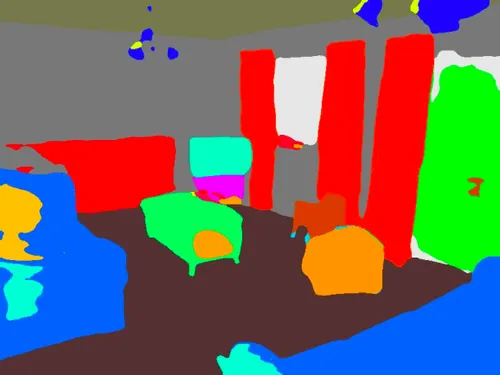
\includegraphics[width=\textwidth]{images/objdet.png}
        \caption{Detecting objects using descriptors}
        \label{fig:desc_objdet}
    \end{subfigure}
    \hfill
    \begin{subfigure}[b]{0.38\textwidth}
        \centering
        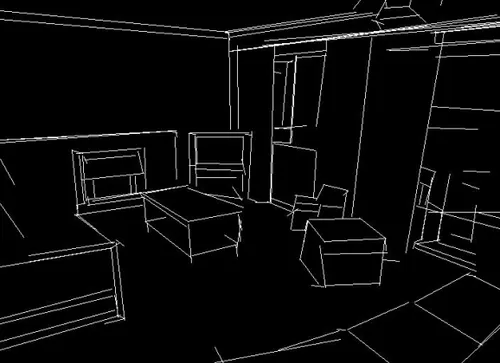
\includegraphics[width=\textwidth]{images/edgedet.png}
        \caption{Identifying edges using descriptors}
        \label{fig:desc_edge}
    \end{subfigure}
    \caption{Data processing using descriptors}
    \label{fig:desc_data}
\end{figure}

Some regions will only be detected once by one specific descriptor. However since we use multiple type of descriptors, more than one descriptor can find the same segment. This would be a problem, however the algorithm uses this to its advantage. It uses the redundant information to determine the easily detectable segments. For the sake of simplicity, in this paper a descriptor detailing a segment is called a representation.

After every possible detail is extracted from an image, we run these representations of segments through a filter that is able to separate the segments into a distinct set. An element of the set consists of a segment and its associated representations. The process of organizing the representations into this set happens by measuring the similarity of two representations against a threshold. If that threshold is reached, the similarity is deemed to be too great and therefore only one of the representation of the segment can remain as the main representation (it is proposed that a high chance of similarity means that the two representations detail the same segment). The unused segment representations are also saved in the set, but only one main representation can be the appointed segment of the set. The process of this filtering is detailed in Algorithm \ref{alg:distinct}, which gives a rough outline of the control and data flow of the algorithm
%algorithm to detail this set creation
\begin{algorithm}
\caption{Building of the Set}\label{alg:distinct}
\begin{algorithmic}
    \State \texttt{Declare set S}
    \State \texttt{Given representations in R}
    \For{ \texttt{representation r in R}}
        \State \texttt{Declare flag F for similarity}
        \For{\texttt{segment s in S}}
            \If{\texttt{r and s similarity > threshold}}
                \State \texttt{Add r as a representation to s}
                \State \texttt{Set F}
                \State \texttt{Raise confidence level of segment s}
            \EndIf
        \EndFor
        \If{F not set}
            \State \texttt{Add r as a segment to s}
            \State \texttt{Initialize confidence level of segment r}
        \EndIf
    \EndFor
\end{algorithmic}
\end{algorithm}


This filtering process also assigns a number to each segment in the set. This number is a so called confidence level, that is able to measure how confident the algorithm is in that this segment is a real, easily distinguishable one. A segment's confidence level is increased if a similar segment was found with a different descriptor. In this case, the algorithm assumes that now more than one descriptor found the same segment and therefore it is more likely that this segment is a real one. 

At the end of this process, we are left with a set of distinct segments, represented by different type of descriptors. Because of the heavy use of different types of feature detection and description, we maximize the number of detectable segments in an image set. The next stage of the process is the association of these segments.

\subsection{Association of the segments} %Segment Association
\label{subsec:assoc_segm}

The first task in the association of segments is determining the interesting and important key points. During the detection phase, some information is already saved about the individual representations, which decriptor found it, how high its activation level was and additional information based on the type of descriptor. While merging them into segments, these characterestics are inherited. Segments also have their confidence score. Based on all these factors, an interest score is calculated for each segment. Then the most important segments will be selected as the first key points.

In the following step, each key point gathers the similar segments around themselves. These groups are also called knots in this paper. An association likeliness score is calculated between each key point and each segment. This includes the similarity of characterestics of the two segments and their disctance. The factors that contributed heavily to the interest score of the key points are weighted more heavily here. Every segment with an association score above a certain threshold is associated with the given key point, it is placed inside its knot. Each segment can be part of multiple knots independently and there is no upper bound for the possible number of association. Therefore, this part of the process can be heavily parallelized to improve the algorithms performance.

These two steps are repreated iteratively. In the following iterations, the number of associations and their strength are also calculated into the interest score of the segments. This ensures that the different segments with different characterestics are selected in each iteration. The desired number of key points and the association threshold are both increased between iterations. While this approach ensures that more and smaller group of segments are gathered around the key points in each iteration, there is no direct hiearchy between them, since the new key points gather segments independently from their previous groups. The iteration of the association ends when a certain number of key points are selected.

This algorithm is summarized in Algorithm~\ref{alg:assoc}.

\begin{algorithm}
\caption{Building of the Knots}\label{alg:assoc}
\begin{algorithmic}
\State \texttt{Declare set K}
\State \texttt{Given segments in S}
\State \texttt{Given desired number of key points as D}
\State \texttt{Given starting association threshold as T}
\State \texttt{Given starting desired number of key points as R}
\While{\texttt{Lenght of K < D}}
    \State \texttt{Declare set P}
    \For{\texttt{segment s in S}}
        \State \texttt{calculate interest score of s}
    \EndFor
    \State \texttt{select R segments from S with the highest interest score into P}
    \For{\texttt{key point k in P}}
        \For{\texttt{segment s in S}}
            \State \texttt{calculate association score a}
            \If{\texttt{a > T}}
                \State {\texttt{associate k and s}}
            \EndIf
        \EndFor
        \State \texttt{add k to K}
    \EndFor
    \State \texttt{increase T}
    \State \texttt{increase R}
\EndWhile
\end{algorithmic}
\end{algorithm}

The next important step is creating a common depiction for each knot. These depictions are also called super segments. To create a super segment, the statistical data for the segments in the knot is calculated. This includes the number of segments and representations in the knot and individual statistics for each characteristic of the segments. For each value the mean, the median, the mode, the quartiles and the deviation are calculated.

Based on these statistics the connection strength score matrix, abbreviated to CSSM, is calculated. The matrix represents the connection strength of every super segment with every other super segment. To get the values for one of the super segments, first the difference between its statistics and every other super segment's is calulated, separately for each characteristic. The differences are ranked and based on the closest value each following one's score is increased. The strength scores are normalized, so for each the closest super segment's score will be one.

\subsection{Defining a layout guess} % Process of recontruction

Taking the aforementioned depictions in the CSSM we attempt to create multiple graph structures that are separate from each other. For a given graph we take the nodes as the depictions. The edges for a given graph differ from graph to graph. These edges are weighted and  determined by a proximity value. If 2 given depictions' strength scores (calculated by the CSSM) are above the proximity value, an edge is formed between the associated nodes. Different graphs work with different proximity values and the strength scores differ from as well. For each graph a proximity value is selected and strength scores are calculated from a CSSM detailed in \ref{subsec:assoc_segm}. This CSSM takes into account different characteristics for each graph. More concretely, every time a different subsection of characteristics are used to define a CSSM. 

The proximity values are selected from a range. This range is defined by taking the CSSM strength scores and setting the range's limits to the first and third quartiles of the strength scores. Proximity values are then picked from this range to be used for the creation of different graphs. The process of defining graphs is detailed in Algorithm \ref{alg:graph}

\begin{algorithm}
\caption{Defining the graphs}\label{alg:graph}
\begin{algorithmic}
\State \texttt{Given depictions in D}
\State \texttt{Given proximity range P}
\State \texttt{Given desired amount of graphs k}
\State \texttt{Define graph G with every depiction from D}
\For{\texttt{k}}
    \State \texttt{Define p proximity value from P}
    \State \texttt{Define CSSM strength scores in matrix C}
    \For{\texttt{depiction d1 in D}}
        \For{\texttt{depiction d2 in D}}
            \If{strength of d1 d2 > p}
                \State \texttt{Create edge between d1 and d2}
            \EndIf
        \EndFor
    \EndFor
\EndFor

\end{algorithmic}
\end{algorithm}


\newpage
As a result of selecting distinct proximity values, we are left with graphs that have various combinations of edges defined. All graphs contain all depictions but the connections of depictioncs is different. The weight of the edges are the strength scores from CSSM. These graphs each define a layout and a relation between depictions, which in turn means it defines a structured layout between grouped segments. These layouts all function as guesses for the true layout, each guess having worked with different proximity value could have a different guess for the layout. Possible outputs resulting in this step can be seen in Figure \ref{fig:layoutguesses}

\begin{figure}[htbp]
    \centering
    \begin{subfigure}[b]{0.38\textwidth}
        \centering
        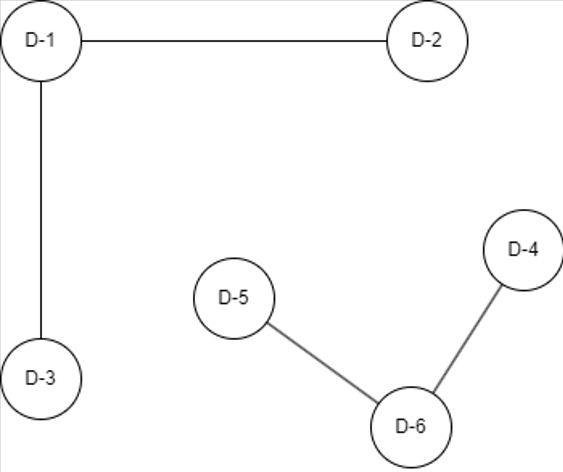
\includegraphics[width=\textwidth]{images/layoutguess1.png}
    \end{subfigure}
    \hfill
    \begin{subfigure}[b]{0.38\textwidth}
        \centering
        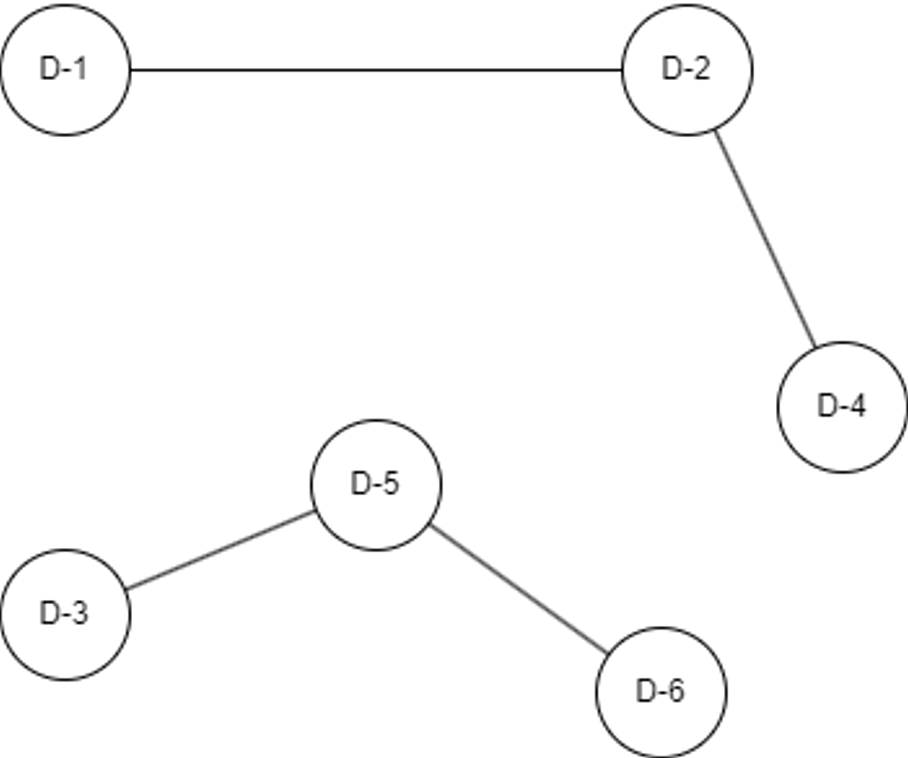
\includegraphics[width=\textwidth]{images/layoutguess2.png}
    \end{subfigure}
    \caption{2 possible layout guesses}
    \label{fig:layoutguesses}
\end{figure}

These graphs are then ran through an algorithm that detects the most commonly guessed edges (and therefore connections). Edges between depictions that are rarely defined are not taken into account. By having different CSSMs for each graph we give a chance for underrepresented edges to also make into the final layout guess. This method of selection produces one final layout that contains the most likely edges.


\subsection{Reconstructing a floor map}

Based on the final layout guess, a floor map can be reconstructed. To achieve this we take the depictions and using the edge characteristics (note that this edge characteristic is given by a descriptor, this is not the graph's edge), we map out an outline of the room. Since the graph's nodes are connected in the appropriate form, we can use the location and edge characteristics to accurately map out a room's walls and corners. Using the locations of the depictions, we could estimate the dimensions of the room. The final representation of a room consists of definition of 2 dimensional points. The corners are represented by points in a cartesian coordinate system, for the sake of simplicity. Coordinates are represented in measures of centimeters. Since doors and windows also have distinct, detectable characteristics, these also get processed as depictions. Using the dimensional data provided by the graph these elements can also be properly placed in a fllor map. For the sake of uniformity, these are also represented as points with a special flag in their data, signaling that these points represent doors and windows.





\section{Results}
\label{sec:results}
We have proven the validity and efficiency of SKBD, by evaluating it on two widely used datasets: Structured3D dataset\cite{zheng2020structured3d} and LSUN dataset\cite{zhang2015large}. We are using a standard metric for evaluation: Corner Error (CE) and Pixel Error (PE). Corner Error is computed by calculating the Euclidean distance between predicted corners and corresponding true corners. Pixel Error is calculated in a similar way, by overlaying the predicted and ground truth polygons, and measuring their difference as a percentage of total image pixels. For the sake of understandability in (fig refs), only wall edges are representing segments, and only wall planes are shown as polygons calculated from knots.

As all other highlighted implementations\cite{8451365}\cite{10350607} focus on Room Layout Reconstruction from a single image, the comparison tests do not fully leverage our solution. However, even in single viewpoint tests our method outperforms already existing state of the art algorithms. For comparison tests, we choose two Convolutional Network based approaches, referred to as MC-FCN\cite{8451365} and HGC\cite{10350607} to use as benchmarks. For MC-FCN, we trained the model based on the DeepLab-ResNet101\cite{chen2017deeplab} architecture. Both competing models were trained on the training subset of each dataset, respectively.


\subsection{Results on Structured3D dataset}
In this test we are using the Strucured3D dataset\cite{zheng2020structured3d}, which is a photo-realistic, large-scale simulated set, containing 3D structure annotations. It consist of 3500 scenes, a total of 21835 rooms and 196515 images, and has a predefined training, validation and test data subset. The input images are resized to \(640 \times 480 \) resolution using bicubic interpolation. For calculating errors, we use the included information about the planes, such as polygon, 3D parameters and semantic label. We evaluate performance between the two proposed models and SKBD using simulated wireframe detection. 

Qualitative results are demonstrated in (fig ref). (fig ref) demonstrates that typical FCNs can sometimes be confused by different surfaces and they might generate incorrect wireframes due to occlusions or clutter. Our method works around these uncertainties by utilizing clearly visible segments around said occlusions, and disregarding segments that have a low confidence level. We summarize the results of the test of set Structured3D in \autoref{table:structured3dperf}. SKBD vastly outperforms both algorithms in Pixel Error and Corner Error metrics.

\begin{table}[H]
\centering
\begin{tabular}{|c | c c |}
    \hline
    Type & $\epsilon[PE](\%)$ & $\epsilon[CE](\%)$ \\ [0.5 ex]
    \hline\hline
    MC-FCN & 6.91 & 4.98 \\
    HGC & 4.17 & 2.57 \\
    \hline
    SKBD & \textbf{1.89} & \textbf{1.34} \\
    \hline
\end{tabular}
\caption{Results on Structured3D dataset}
\label{table:structured3dperf}
\end{table}


\subsection{Results on LSUN dataset}
For this test we are using the relabeled LSUN dataset released by \cite{ren2017coarse}. The dataset consists of 4000 training images, 394 validation images and 1000 testing images. We manually grouped the images taken of the same room from multiple angles, and resized all images to \( 640 \times 480 \) resolution. Ground truth polygon edges and corner points were pre-calculated using the depth and normalmaps included in the dataset, but the input of the algorithms only includes the RGB data. The dataset also provides an official toolkit which suggest the usage of Pixel Error and Corner Error metrics that we also used for the Structured3D set.

This dataset only consists of images of rooms that conform to the Manhattan World Assumption\cite{790349} which favors MC-FCN and HGC. The overall quality of the images are worse compared to the Structured3D set, with more variation in image exposure and more occluions over corners and wall edges. This caused all three algorithms to perform worse, however SKBD still outperforms both MC-FCN and HGC as summarized in \autoref{table:lsunperf}.

\begin{table}[H]
\centering
\begin{tabular}{|c | c c |}
    \hline
    Type & $\epsilon[PE](\%)$ & $\epsilon[CE](\%)$ \\ [0.5 ex]
    \hline\hline
    MC-FCN & 8.91 & 6.75 \\
    HGC & 5.29 & 3.44 \\
    \hline
    SKBD & \textbf{3.17} & \textbf{2.41} \\
    \hline
\end{tabular}
\caption{Results on LSUN dataset}
\label{table:lsunperf}
\end{table}





\section{Discussion}
\label{sec:discussion}

The results obtained from the experiments on both the Structured3D and LSUN datasets provide significant insights into the effectiveness of our proposed SKBD method compared to state-of-the-art approaches. One of the most notable findings is the considerable improvement in both Pixel Error (PE) and Corner Error (CE) metrics when utilizing multiple viewpoints. SKBD outperformed all available solutions on both datasets that were introduced in Results \ref{sec:results}. For dataset Structured3D SKBD achieved a PE and CE score of under 1\%. For dataset LSUN, the results were still more optimal than other solutions, achieving a PE and CE score of under 1.5\%

This demonstrates that SKBD is capable of efficiently leveraging multi-view image data, which is a key differentiator from methods that rely on single images.

\subsection{Multi-Viewpoint Advantage}
The results obtained from the Structured3D dataset emphasize the significant advantages of employing a multi-viewpoint strategy in room reconstruction. SKBD's ability to integrate data from multiple angles allows for a more comprehensive understanding of the scene, which is especially beneficial in overcoming challenges that single-view methods often face. For example, occlusions where certain parts of the room are hidden from view—or clutter, which obscures crucial features, typically introduce inaccuracies in methods like MC-FCN and HGC. However, SKBD’s multi-viewpoint approach minimizes these issues by piecing together visual information from different perspectives, resulting in a more accurate and detailed reconstruction. This capability is especially crucial when dealing with non-cuboid or irregularly shaped rooms, where accurate detection and connection of segments from various viewpoints can make a significant difference. Our experimental results demonstrate this advantage, as the multi-viewpoint tests achieved a PE of 0.77\% and a CE of 0.68\%, marking a substantial improvement over competing methods.

\subsection{Handling of Occlusions and Irregular Surfaces}
A key strength of SKBD is its robust handling of occlusions and irregular room layouts, as highlighted by the qualitative results (Figure \ref{fig:comparisontest}). Traditional methods, such as MC-FCN and HGC, tend to perform poorly when faced with rooms featuring occlusions, clutter, or non-cuboid geometries, leading to higher error rates. These methods are often designed with cuboid rooms in mind, and as such, struggle when applied to more complex layouts. In contrast, SKBD excels in such scenarios due to its focus on segment knotting and boundary detection. By accurately detecting boundaries and associating segments, SKBD can reconstruct irregularly shaped rooms with far greater precision, even when certain areas are obscured or contain complex surfaces. This capacity to handle occlusions and unusual geometries significantly enhances its performance compared to conventional methods.

\subsection{Generalizability Across Datasets}
The generalizability of SKBD is another key advantage, as demonstrated by its consistent performance across different datasets. In addition to excelling on the Structured3D dataset, SKBD also performs well on the LSUN dataset, despite the latter’s more challenging image quality and adherence to the Manhattan World Assumption. While the LSUN dataset presents greater difficulty due to lower image quality and more complex environments, SKBD still outperforms MC-FCN and HGC, though with slightly higher error rates. This demonstrates that SKBD is not limited to simulated, high-quality datasets but is also capable of effectively handling real-world data with more variation in structure and visual quality. The PE and CE on the LSUN dataset, at 1.13\% and 1.06\%, respectively, further illustrate SKBD’s superior performance across diverse environments, maintaining its edge over competing approaches.

\subsection{Limitations}
While SKBD has shown significant improvements over existing methods, there are several limitations that need to be addressed. First, the method’s reliance on high-quality input images limits its applicability in scenarios with lower resolution or noisy data, such as images taken in poor lighting conditions or with low-quality cameras. The accuracy of the reconstructed room layouts decreases noticeably when the image quality is suboptimal, which can affect the overall performance of the system, particularly on real-world datasets where ideal conditions cannot always be guaranteed.

Second, SKBD's multi-viewpoint strategy, while advantageous in many cases, may not be as effective in environments with extreme occlusions or significant clutter. In such situations, the algorithm may struggle to detect and connect segments accurately, leading to potential inaccuracies in the final reconstruction. 

Additionally, SKBD is currently optimized for non-cuboid room geometries, which means that its performance in cuboid rooms may not be fully realized. This specialization could limit its application in simpler scenarios where cuboid layouts are more common.

Lastly, while the algorithm performs well under the Manhattan World Assumption, many real-world environments do not conform to this constraint. This limitation may restrict SKBD's applicability in more complex spatial arrangements found in actual buildings.


\section{Conclusion}
\label{sec:conclusion}
The problem presented in this paper was the problem of reconstructing a room into its floor map with as few images taken as possible. We wanted to cover cuboid and non-cuboid shaped rooms, even if it came with taking more than one image as the source of reconstruction. More than one method was tried in order to achieve the outcome, which are detailed in the methodology section \ref{sec:methodology} for the purpose of transparency and clarity of what methods did not work. We presented our solution in a way that allows anyone interested in the topic to reproduce our research. When presenting our results\ref{sec:results} we found that our solution was able to perform at a desirable level. It outperforms known solutions on multiple databases. Our solution also enhances usability by providing output data that is easy to process. Using our method various services and applications can be developed and used. We managed to create a system in which a room's floor plan can be reliably reconstructed and processed for further use. This system not only improves on known methods but also opens up new possibilities for applications that depend on efficient and accurate spatial mapping.

\section{Future Work}


\listoffigures

\listoftables

\listofalgorithms

\printbibliography           % Produces references

\end{document}               % End of document.